% lark-eunis16.tex
% 

\ifdefined\handout         % ----- IEEE HPEC conference proceedings

\documentclass[ignorenonframetext,handout]{beamer}

\else

\documentclass[ignorenonframetext]{beamer}

\fi

% -------------------- PREAMBLE

% ----- customizations

% preamble-packages.tex


% fix booktabs compatibility issue
\usepackage{etex}
\usepackage{animate}

% math
\usepackage{sansmathaccent}
\usepackage{amsmath}
\usepackage{amssymb}
\usepackage{mathrsfs}
\usepackage{array}


% graphics
\usepackage[font=small,compatibility=false,justification=centering]{caption}
\usepackage[font=small,labelformat=empty,justification=centering]{subcaption}
\usepackage{graphicx}
\usepackage{tikz}

\usepackage{dirtree}

% tables
\usepackage{multirow}
\usepackage{booktabs}

% fonts
\usepackage{natbib}
\usepackage{todonotes}

\usepackage{textpos}

\usepackage{microtype}

\usepackage{grffile}

% for Android theme
\usepackage{bold-extra}
\usepackage{listings}


% directory path
\usepackage{menukeys}

%%% Local Variables:
%%% mode: latex
%%% TeX-master: "../android-studio-main"
%%% End:

% preamble-extras.tex
%
%

\usetheme[bullet=circle,% Use circles instead of squares for bullets.
          titleline=true,% Show a line below the frame title.
          alternativetitlepage=true,% Use the fancy title page.
          titlepagelogo=figs/android-logo,% Logo for the first page.
          watermark=figs/android-watermark,% Watermark used in every page.
          watermarkheight=100px,% Height of the watermark.
          watermarkheightmult=4,% The watermark image is 4 times bigger
                                % than watermarkheight.
          ]{Android}


\lstset{language=Java,captionpos=b,
tabsize=4,frame=lines,
basicstyle=\scriptsize\ttfamily,
keywordstyle=\color{blue},
commentstyle=\color{lightgray},
stringstyle=\color{violet},
breaklines=true,showstringspaces=false}

\AtBeginSection[]{%
  \begin{frame}<beamer>
    \frametitle{Outline}
    \tableofcontents[currentsection]
  \end{frame}
  \addtocounter{framenumber}{-1}% If you don't want them to affect the slide number
}



%%% Local Variables:
%%% mode: latex
%%% TeX-master: "../android-studio-main"
%%% End:
% preamble-customizations.tex


% fix Linux Adobe Acrobat Reader's issue with transparent image elements
% \pdfpageattr{/Group << /S /Transparency /I true /CS /DeviceRGB>>}


% define coloured clickable links
\hypersetup{%
  pdffitwindow=false,%
  pdfstartview={FitH},%
  % colorlinks,%
  pdfauthor={},%
  pdftitle={},%
  pagebackref=true,%
  citecolor=PaleGreen4,%
  filecolor=DarkOrchid4,%
  % linkcolor=OrangeRed4,%
  urlcolor=RoyalBlue4%
}

% define the includegraphics search path
\graphicspath{%
  {figs/}%
}

% short-hand command for hyperlinked e-mails
\newcommand{\email}[1]{\href{mailto:#1}{\texttt{#1}}}

% redefine \boxed command to allow setting the border color
\newcommand{\highlight}[1]{\fcolorbox{complclr1}{white}{$\displaystyle #1$}}

% modified bullet-point for highlighting
\newcommand{\bulletemph}{$\large\boldsymbol{\star}$}

% command to output names under images
\newcommand{\imentry}[3][1.25cm]{%
  \vbox{\halign{\hfil##\hfil\cr%
      \includegraphics[height=#1]{#2}\cr#3\cr}}}

\definecolor{custom_theme}{HTML}{91043D}

%%% Local Variables:
%%% mode: latex
%%% TeX-master: "../android-studio-main"
%%% End:


\sloppy

% ---------- DATE
% 

\newcommand{\datestring}{Mar. 20, 2017}
\date%
[\datestring]%
{\footnotesize \datestring}

% ---------- TITLE
%
\title%
[Android Studio Development]%
{ Android Development using Android Studio% \\
  % \emph{Learning with Computer-Assisted Guided Tours}%
}


% ---------- CONFERENCE
%
\subtitle%
{ \footnotesize BEST Mobile App Development }



% ---------- AUTHORS
%
\author%
[\emph{D. Floros}, K. Mylonakis]%
{%
  \imentry{dimitris-floros.png}{\emph{Dimitris Floros}} \and%
  \imentry{kostas-mylonakis.png}{Kostas Mylonakis}%
}


% ---------- AFFILIATIONS
\institute%
[]%
{%
  Department of Electrical and Computer Engineering,
  Aristotle University of Thessaloniki%
}



% -------------------- MAIN MATTER

\begin{document}
\frame[plain]{\titlepage}

\frame{\tableofcontents[]}

\mode<all>

%---- INTRODUCTION --------

\section{Introduction}
\label{sec:introduction}

% general introduction
% introduction.tex
%
%

\begin{frame}
  \frametitle{What is Android?}
  
  \begin{itemize}
    
  \item<1-> Android represents an exciting new oppurtinity to write
    innovative applications for smartphones
  \item<2-> Android is an \emph{open-source} stack that includes
    \begin{itemize}
    \item<3-> Operating system
    \item<3-> Middleware
    \item<3-> API libraries
    \end{itemize}
    
  \item<3-> Powered by Linux operating system

  \item<4-> Fast application development in Java

  \end{itemize}

\end{frame}



%%% Local Variables:
%%% mode: latex
%%% TeX-master: "../android-studio-main"
%%% End:


% android devices possibilities
% android-devices.tex
%
%

\begin{frame}
  \frametitle{Android devices}
  
  Modern mobile smart-phones have become powerful tools

  \begin{itemize}
  \item<2-> Cameras
  \item<3-> WiFi -- 4G
  \item<4-> GPS system
  \item<5-> Sensors
    \begin{itemize}
    \item<6-> Accelerometer
    \item<6-> Gyroscope
    \item<6-> Magnetometer
    \end{itemize}
  \end{itemize}
  
  \onslide<7->{
    New possibilities in \emph{application development}
  }

\end{frame}

%%% Local Variables:
%%% mode: latex
%%% TeX-master: "../android-studio-main"
%%% End:

%  LocalWords:  Accelerometer


% online resources
% online-resources.tex
%
%

\begin{frame}
  \frametitle{Online resources}
  
  \begin{itemize}
  \item<1-> Android Developers
    \begin{itemize}
    \item \url{http://developer.android.com}
    \end{itemize}
  \item<2-> Android Studio -- SDK
    \begin{itemize}
    \item \url{http://developer.android.com/sdk/index.html}
    \end{itemize}
  \item<3-> Google Play Store
    \begin{itemize}
    \item \url{ https://play.google.com/store }
    \end{itemize}
  \end{itemize}

\end{frame}

%%% Local Variables:
%%% mode: latex
%%% TeX-master: "../android-studio-main"
%%% End:



% ---------- ANDROID PLATFORM

\section{Android Platform}
\label{sec:android-platform}

% image showing Android stack
% android-stack.tex
%
%


\begin{frame}[plain]

  \begin{figure}
    \centering
    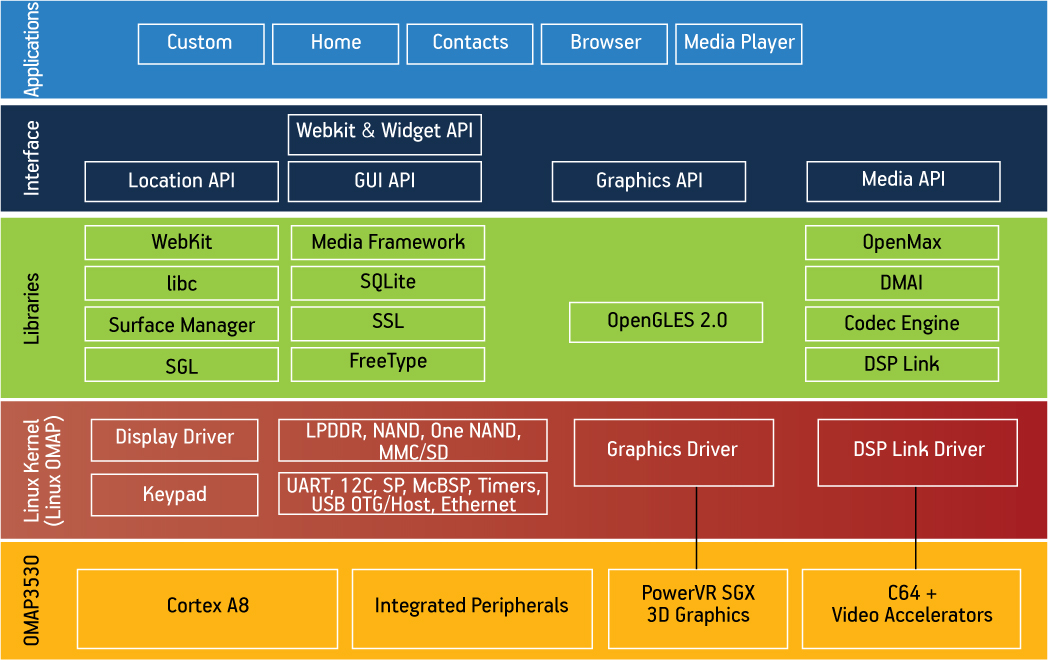
\includegraphics[height=0.8\textheight]{android-application-stack}
    \caption{Android Software Stack on OMAP3530 \\
      \emph{Source}: Texas Instruments}
    \label{fig:android-stack}
  \end{figure}
  
\end{frame}


%%% Local Variables:
%%% mode: latex
%%% TeX-master: "../android-studio-main"
%%% End:


% linux kernel
% linux-kernel.tex
%
%


\begin{frame}
  \frametitle{Linux Kernel}
  
  \begin{itemize}
  \item<1-> Works as a HAL (Hardware Abstraction Layer)
  \item<2-> Device drivers
  \item<3-> Memory management
  \item<4-> Process management
  \item<5-> Networking
  \end{itemize}

  \begin{figure}
    \centering
    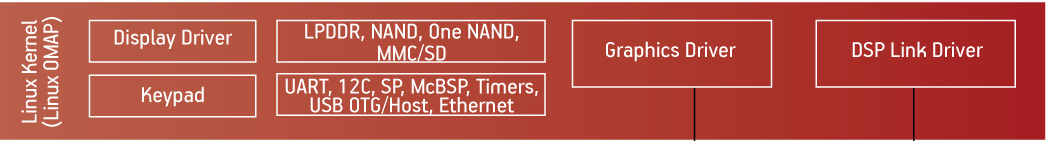
\includegraphics[width=\textwidth]{android-application-stack-linux-kernel}
  \end{figure}


\end{frame}


%%% Local Variables:
%%% mode: latex
%%% TeX-master: "../android-studio-main"
%%% End:


% libraries
% libraries.tex
%
%


\begin{frame}
  \frametitle{Libraries}
  
  \begin{itemize}
  \item<1-> C/C++ libraries
  \item<2-> Interface through Java
  \item<3-> Surface manager -- Handling UI Windows
  \item<4-> 2D and 3D graphics
  \item<5-> Media codecs, SQLite, Browser engine
  \end{itemize}

  \begin{figure}
    \centering
    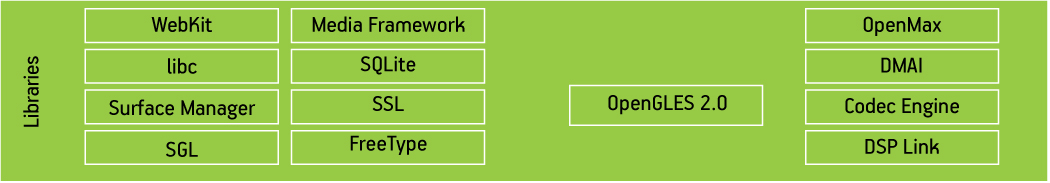
\includegraphics[width=\textwidth]{android-application-stack-libraries}
  \end{figure}


\end{frame}


%%% Local Variables:
%%% mode: latex
%%% TeX-master: "../android-studio-main"
%%% End:


% ---------- PLATFORM ARCHITECTURE

\section{Platform Architecture}
\label{sec:platform-architecture}


% ---------- BUILDING BLOCKS

\section{Building Blocks}
\label{sec:building-blocks}


% ---------- ANDROID STUDIO

\section{Android Studio}
\label{sec:android-studio}

% ---------- HELLO ANDROID

\section{Hello Android Application}
\label{sec:hello-android}


% ---------- ACKNOWLEDGMENTS

\section{Acknowledgments}
% acknowledgment.tex
%
%
%

\begin{frame}[plain]
  \frametitle{Acknowledgment}
  \begin{tabular}{cl}  
    \begin{tabular}{c}
      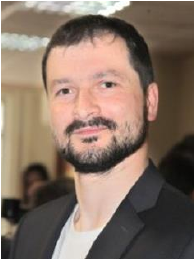
\includegraphics[height=0.25\textheight]{spiros-bond.png}%
    \end{tabular}
    & 
      \begin{tabular}{l}
        \parbox{0.75\linewidth}{%  change the parbox width as appropiate
        \emph{Spiros Bontomitsidis} for his critical comments
        }
      \end{tabular}  \\
  \end{tabular}
  
  \vspace{2em}
 
  
\end{frame}



%%% Local Variables:
%%% mode: latex
%%% TeX-master: "../android-studio-main"
%%% End:


% ================= references =========================

\nocite{*}
\mode*
\appendix
\backupbegin
\begin{frame}[plain, allowframebreaks]
    \frametitle{References}
    \bibliographystyle{abbrvnat}
    {\tiny \bibliography{ref.bib}}
\end{frame}
\backupend

\end{document}




%%% Local Variables:
%%% mode: latex
%%% TeX-master: t
%%% End:
